\documentclass[spanish,xcolor=table,svgnames]{beamer}
\definecolor{mediumpurple4}{rgb}{0.36,0.28,0.55}
%colores coporativos
\definecolor{naranja}{rgb}{0.86,0.42,0.06}
\definecolor{gris}{rgb}{0.41,0.41,0.41}
\definecolor{azul}{rgb}{0.06,0.31,0.55}
\definecolor{rojo}{rgb}{1,0,0}
\definecolor{azulito}{RGB}{122,189,255}
\definecolor{naranjita}{RGB}{255,183,99}
\usepackage[spanish]{babel}
\AtBeginDocument{
\renewcommand{\tablename}{Tabla}
\def\changemargin#1#2{\list{}{\rightmargin#2\leftmargin#1}\item[]}
\let\endchangemargin=\endlist
}

%\beamertemplateshadingbackground{white}{naranjita!10} % degradado de amarillo a magenta

\setbeamercolor{title}{fg=black,bg=black!20}
%\setbeamercolor{block title example}{fg=white,bg=blue!90}
%\setbeamercolor{block title alerted}{fg=white,bg=blue!90}
%\setbeamercolor{block body alerted}{fg=blue!90,bg=white}

%\setbeamercolor{title}{fg=red!80!black,bg=red!20!white}
%\setbeamerfont{}{shape=\itshape,family=\rmfamily}
\mode<presentation>
{

  %\usetheme{Copenhagen}
%\usetheme{Luebeck}
\usetheme{Warsaw}
%\useoutertheme{infolines}
 % \setbeamertemplate{navigation symbols}{}
  \setbeamertemplate{title page}[rounded=true,shadow=true]
\setbeamercolor{structure}{fg=naranjita}
\setbeamercolor{section in head/foot}{bg=azulito}
}
\usepackage[spanish]{babel}
\usepackage[utf8x]{inputenc}
\usepackage{charter}
\usepackage[T1]{fontenc}
\usepackage{fancyvrb}
\usepackage{tikz}
%\usepackage{microtype}
\usepackage{xspace}
\usepackage{ctable}
\usepackage{alltt,multicol}

\newcommand{\reduce}{\fontsize{8}{9}\selectfont}
\graphicspath{{./img/}} 
%\usetikzlibrary{chains,positioning,decorations.pathreplacing,fit,scopes}

\title[Optinet: Software de Gestión Web para centros Ópticos]{Optinet \\ Software de Gestión Web para centros Ópticos}
\author{José Ángel Parada Jiménez}
\institute[UCA]{Ingeniería Técnica en Informática de Gestión \\ Universidad de Cádiz}
\date{28 de junio de 2013} %poner la fecha

\DefineVerbatimEnvironment{vrbwithcmd}{Verbatim}{commandchars=+(),fontsize=\small}

\begin{document}

\begin{frame}
  \titlepage
  \begin{figure}
	
\includegraphics[height=0.2\textheight]{logo_uca} 
  \end{figure}
\end{frame}

\frame{\frametitle{Índice}\tableofcontents}

\section{Introducción}
\frame{\tableofcontents[currentsection]}

\subsection*{Empresa Salud visión}
\frame{\frametitle{Salud visión}
\begin{itemize}
\item Petición por parte del gerente de Salud Visión S.L. construir un sistema de gestión.
\item Interés personal por el desarrollo de un software de gestión.
\item Interés personal por programación web.
\end{itemize}
  \begin{figure}
       
\includegraphics[scale=0.6]{saludvision}
\end{figure}
}

\subsection*{Localización Salud Visión}
\frame{\frametitle{Localización}
Salud Visión S.L.
  \begin{figure}
 	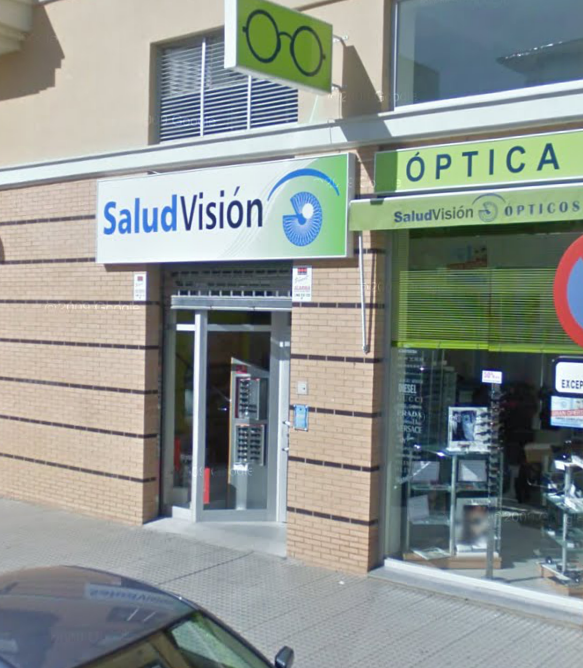
\includegraphics[scale=0.23]{capcalle2}\hspace{5mm}
	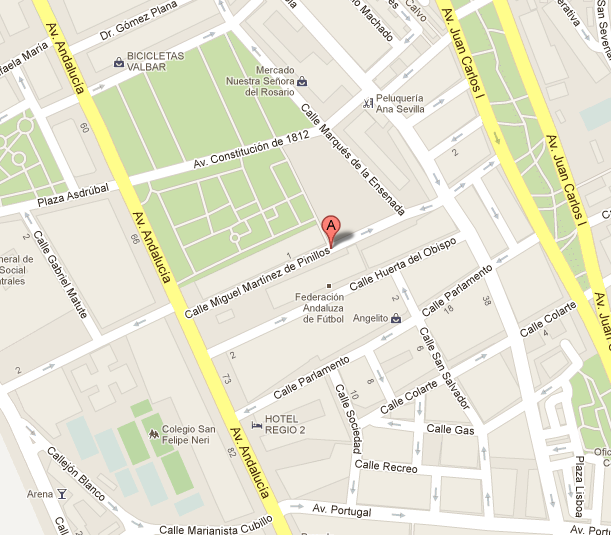
\includegraphics[scale=0.25]{mapa}
\end{figure}
}

\subsection*{Software actual}
\frame{\frametitle{Software Actual}
  \begin{figure}
	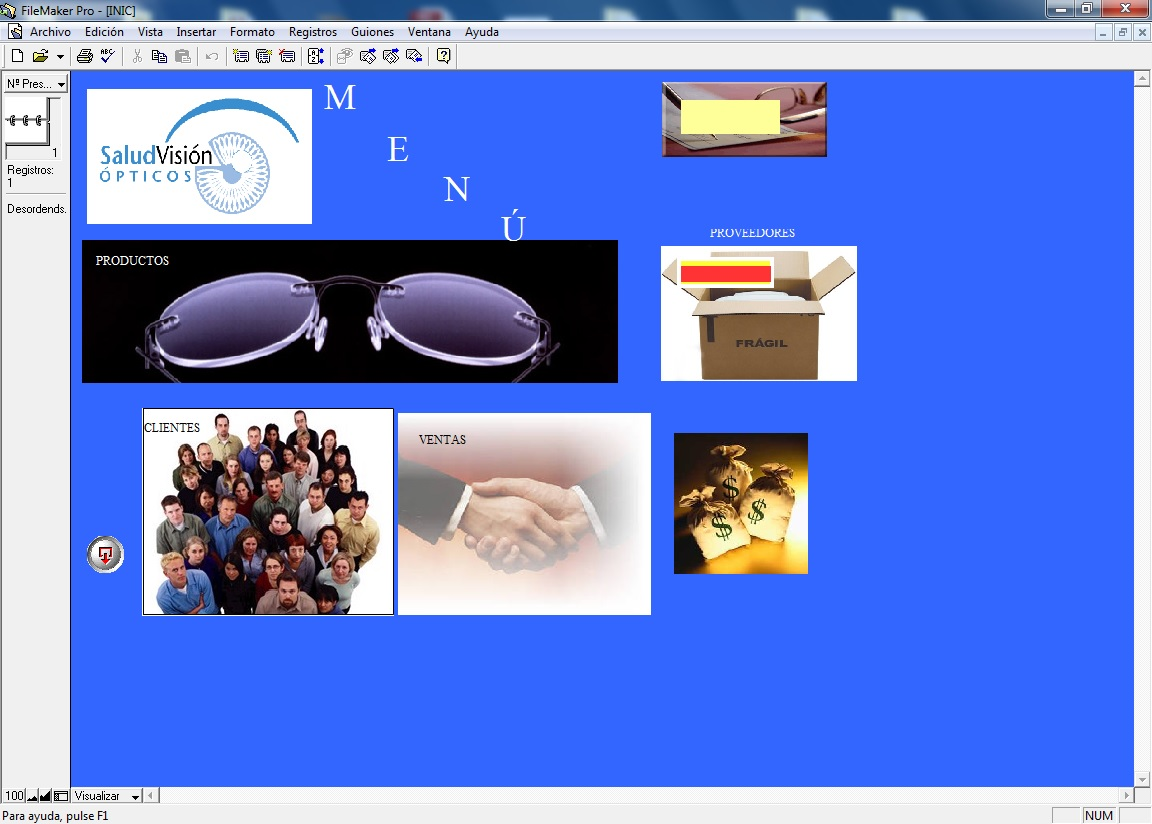
\includegraphics[scale=0.18]{menu}
\end{figure}\pause
\begin{block}{Problemas}
\begin{itemize}
\item Aspecto visual.
\item Problema de usabilidad.
\item Carencias de funcionalidades.
\end{itemize}
\end{block}
}

\subsection*{Objetivos del proyecto}
\frame{\frametitle{Objetivos del proyecto}
  \begin{figure}
 	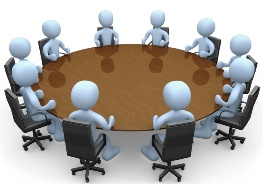
\includegraphics[scale=0.23]{reuniones}
\end{figure}
\begin{block}{Objetivos principales}
\begin{itemize}
\item Construir aplicación web para gestionar un centro óptico.\\\pause
\item Gestión de productos, proveedores, pedidos, ventas...\\\pause
\item Generar informes.\\\pause
\item Control de las acciones que realizan los usuarios.\\\pause
\item Multi-idioma y multi-plataforma.\\\pause
\item Segura, fiable y tener un rendimiento adecuado.
\end{itemize}
\end{block}
}


%%%%%%%%%%%%%%%%%%%%%%%%%%%%%%%
\section{Desarrollo del proyecto}
\frame{\frametitle{Desarrollo del proyecto}\tableofcontents[currentsection]}

\subsection*{Calendario y metodología}

\frame{
\frametitle{Metodología}
\begin{center}
    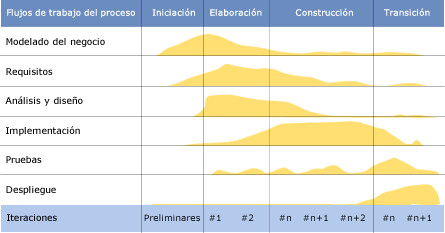
\includegraphics[width=0.7\textwidth]{Rup}
\end{center}
\begin{itemize}
\item Se ha utilizado la metodología RUP al ser la más utilizada para la construcción de sistemas orientados a objetos.
\item En cada fase participan todas las disciplinas, pero dependiendo de la fase el esfuerzo dedicado a una disciplina varía.
\end{itemize}
}

\frame{
\frametitle{Calendario}
    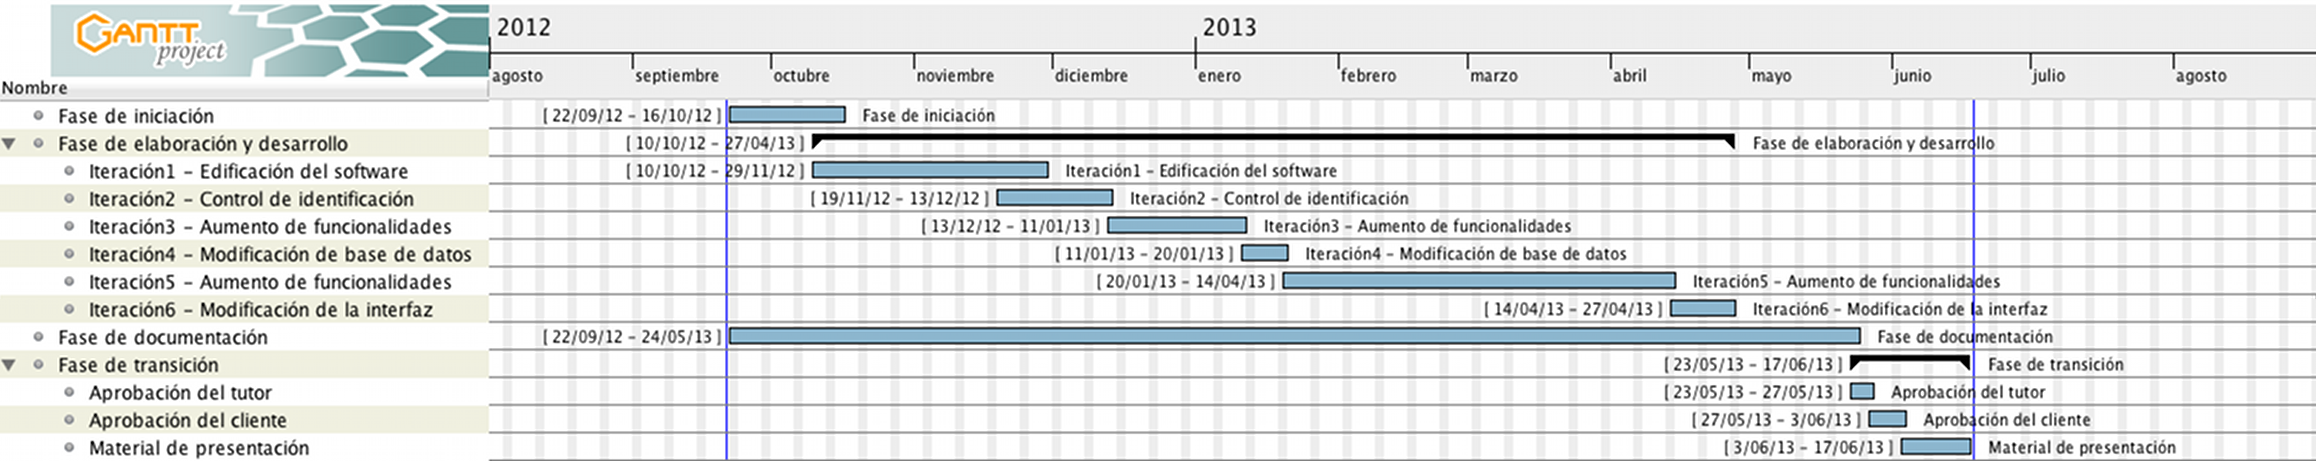
\includegraphics[width=1\textwidth, height=0.45\textheight]{gantt1}
}


\frame{
\frametitle{Estimación de tiempos}
\begin{table}[ht]
\centering  % used for centering table
\begin{tabular}{c c c} % centered columns (4 columns)
\hline\hline                        %inserts double horizontal lines
Fase & Tiempo estimado & Tiempo real \\ [0.5ex] % inserts table 
%heading
\hline                  % inserts single horizontal line
Fase de iniciación & 60 horas & 75 horas  \\ % inserting body of the table
Fase de elaboración y construcción & 400 horas & 550 horas \\
Fase de documentación & 30 horas &  50 horas\\
Fase de transición & 50 horas & 70 horas  \\   [1ex]      % [1ex] adds vertical space
\hline
Total & 540 horas & 745 horas  \\
\end{tabular}
\end{table}
  \begin{block}{}
Se realizó la planificación de los tiempos de las tareas pero no se cumplieron debido a problemas no esperados o dificultad añadida no prevista.
  \end{block}
}


\subsection*{Análisis}
\begin{frame}{Requisitos Software}
  \begin{block}{}
\begin{itemize}
\item Control de acceso y roles de los usuarios.\pause
\item Organización de los productos agrupados por familias.\pause
\item Creación de documentos e informes con el logotipo.\pause
\item Control de los proveedores del sistema.\pause
\item Control de las citas que se generen.\pause
\item Control de los pedidos, ventas, devoluciones, reservas y apartados que generen los usuarios.\pause
\item Control de los informes que se generen.\pause
\item Control de los cambios realizados en el sistema.\pause
\item Control de los arqueos realizados en el sistema.\pause
\item Control de los permisos disfrutados por los usuarios.
\end{itemize}
  \end{block}
\end{frame}

\begin{frame}{Actores del sistema}

Se definieron las distintas responsabilidades de los usuarios del sistema quedando de la siguiente manera:\\
\begin{table}[ht]
\begin{tabular}{c c c c} % centered columns (4 columns)
\hline\hline                        %inserts double horizontal lines
 & Administrador & Empleado & Médico\\ [0.5ex] % inserts table 
%heading
\hline                  % inserts single horizontal line
Gestión operaciones & X & X & X  \\ % inserting body of the table
Ver informes & X & X & X \\
Crear informes & - & - & X  \\
Administración & X & - & -  \\   [1ex]      % [1ex] adds vertical space
\hline
\end{tabular}
\end{table}
\end{frame}

\subsection*{Diseño}
\begin{frame}{Arquitectura física}
  \begin{figure}[]
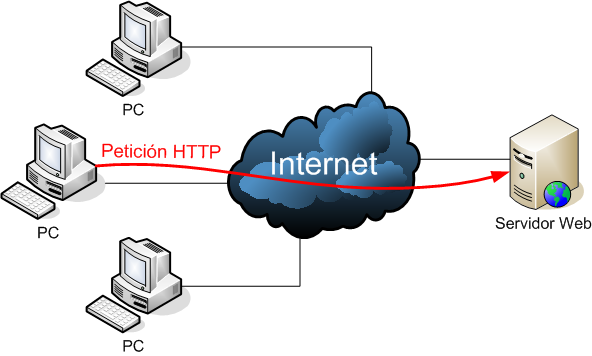
\includegraphics[scale=0.35]{arquitectura}
\end{figure}
  \begin{block}{}
Varios usuarios trabajando sobre la aplicación simultáneamente.
  \end{block}
\end{frame}

\begin{frame}{Arquitectura lógica}

\begin{columns}[c]
\column{0.4 \textwidth}
  \begin{figure}[]
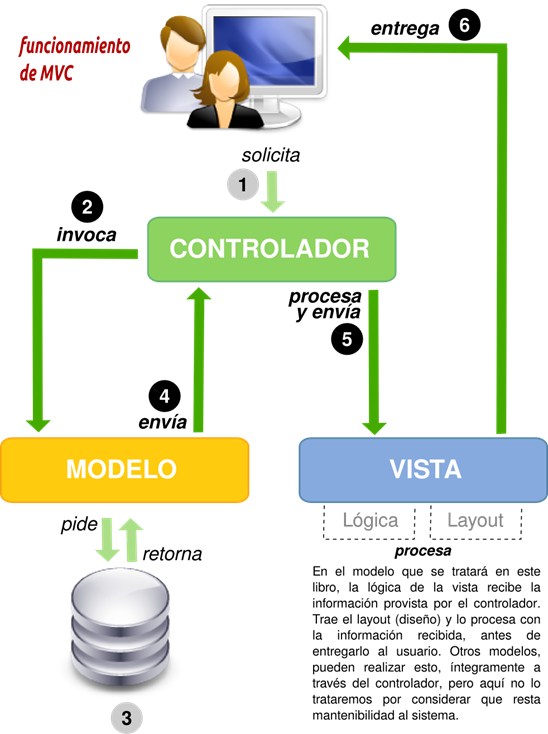
\includegraphics[scale=0.3]{mvc}
\end{figure}
\column{0.6 \textwidth}
  \begin{block}{}
 El patrón MVC es una arquitectura de diseño software para separar los componentes de aplicación en tres niveles, interfaz de usuario, 
lógica de control y lógica de negocio.
  \end{block}
\end{columns}
\end{frame}

\begin{frame}{Diseño}
  \begin{figure}[]
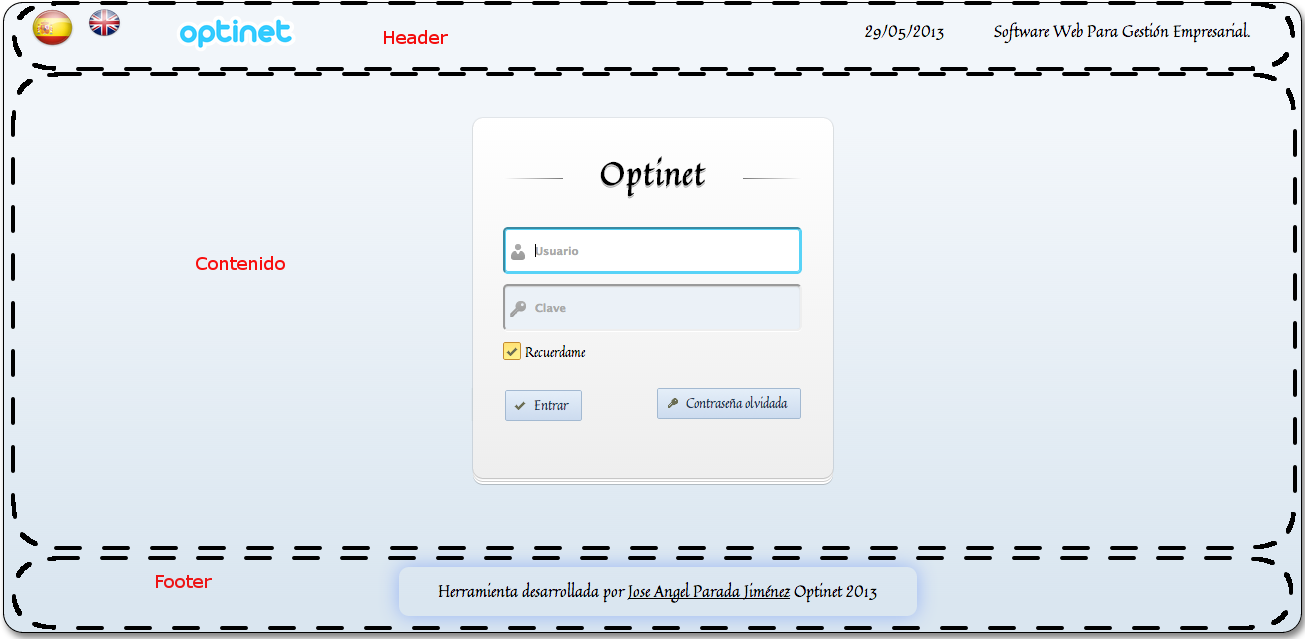
\includegraphics[scale=0.2]{diseno}
\end{figure}
  \begin{block}{}
 Antes de llegar al diseño definitivo de la imagen se crearon bocetos con la herramienta Pencil App. 
  \end{block}
\end{frame}

\subsection*{Implementación}
\frame{\frametitle{Implementación}
  \begin{block}{}
 \begin{itemize}
\item Se realizó un estudio del entorno de trabajo para la construcción de la aplicación.
\item Se barajaron diferentes lenguajes de programación PHP, JSP, ASP
\item Se eligió PHP ( rapidez, documentación, variedad de módulos, similar a C, especializado para web...)
\item Una vez elegido el lenguaje, se estudiaron los diferentes frameworks de PHP: Codeigniter, Symfony, Yii, CakePHP.
\end{itemize}
  \end{block}
}
\frame{\frametitle{Lenguajes utilizados}
  \begin{figure}[]

\includegraphics[scale=0.2]{php}\hspace{9mm}
 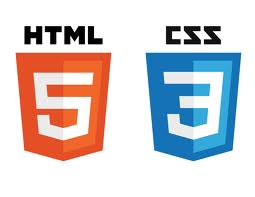
\includegraphics[scale=0.3]{htmlcss}
\end{figure}

  \begin{figure}
       
\includegraphics[scale=0.85]{javascript}\hspace{4mm}
\end{figure}

}

\frame{\frametitle{Frameworks utilizados}

  \begin{figure}[]

\includegraphics[scale=0.4]{symfony2}
\end{figure}
  Symfony2 es un framework de PHP rápido, flexible y fácil de aprender que nos permite a los desarrolladores construir aplicaciones webs más mantenibles.

  \begin{figure}[]
 
\includegraphics[scale=0.1]{jquery}
\end{figure}
  jQuery es un framework de JavaScript, que permite simplificar la manera de interactuar con los documentos HTML, manipular el árbol DOM, manejar eventos, desarrollar animaciones (FLV) y agregar interacción con la técnica AJAX a páginas web.

}

\begin{frame}{Descripción de los frameworks}
 \begin{block}{Características Symfony2}
  \begin{itemize}
\item \textbf{Versátil}
\item \textbf{Seguridad} 
\item \textbf{Flexible} 
\item \textbf{Rendimiento} 
\item \textbf{Soporte} 
\item \textbf{Documentación} 
\item \textbf{Comunidad} 
\item \textbf{Popular}
\end{itemize}
  \end{block}
\end{frame}

\begin{frame}{Descripción de los frameworks}
 \begin{block}{Caracteristicas jQuery}
  \begin{itemize}
\item Selección, interactividad y modificaciones del árbol DOM.
\item Eventos.
\item Manipulación de la hoja de estilos CSS.
\item Efectos y animaciones.
\item Animaciones personalizadas.
\item AJAX.
\item Soporta extensiones.
\item Gran compatibilidad con navegadores.
\end{itemize}
  \end{block}
\end{frame}


\frame{\frametitle{Bibliotecas utilizadas}

  \begin{figure}[]
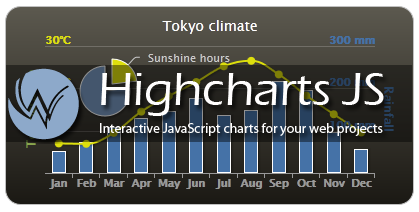
\includegraphics[scale=0.25]{highcharts}\hspace{6mm}
 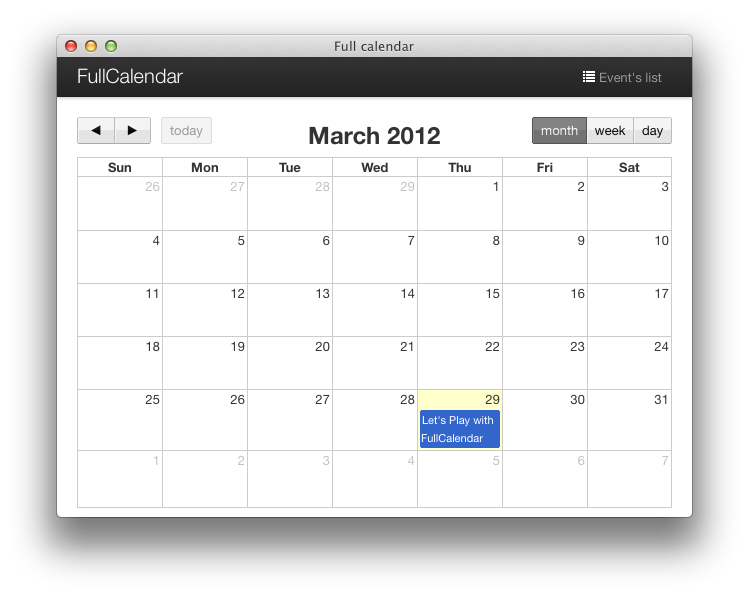
\includegraphics[scale=0.1]{fullcalendar}\hspace{2mm}

\includegraphics[scale=0.35]{datatables}
\end{figure}

  \begin{figure}
       
\includegraphics[scale=0.2]{jqueryui}\hspace{9mm}
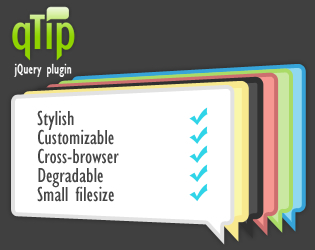
\includegraphics[scale=0.2]{qtip}\hspace{4mm}

\includegraphics[scale=0.2]{fphp}
\end{figure}

}



\frame{\frametitle{Entorno de trabajo}
  \begin{figure}[]

\includegraphics[scale=0.5]{lamp}\hspace{10mm}

\includegraphics[scale=0.2]{pencil}\hspace{10mm}

\includegraphics[scale=0.05]{latex}\\

\includegraphics[scale=0.3]{git}\hspace{30mm}

\includegraphics[scale=0.25]{ganttlogo}\\

\includegraphics[scale=1.2]{dia}\hspace{15mm}
\fbox{
\includegraphics[scale=0.2]{ubuntu}}\hspace{15mm}

\includegraphics[scale=0.25]{gimp}\\

\includegraphics[scale=0.15]{sublime}\hspace{30mm}

\includegraphics[scale=0.15]{textworks}
\end{figure}
}

\frame{\frametitle{Flujo de una petición en Symfony2} 
  
\begin{figure}[]
 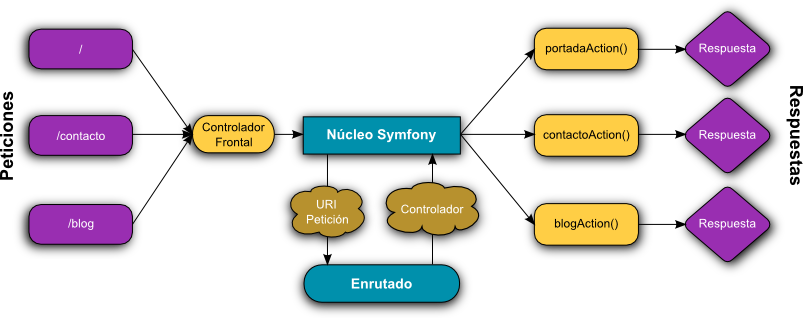
\includegraphics[scale=0.4]{peticiones}
\end{figure}
}

\frame{\frametitle{Modelo - Vista - Controlador}
 Modelo: Representa los datos de la aplicación.
\begin{itemize}
\item Se hace uso del ORM doctrine para convertir las tablas de nuestra base de datos en clases y los registros en objetos que podemos manejar con facilidad.
\end{itemize}
\begin{figure}[]
 
\includegraphics[scale=0.4]{doctrine}
\end{figure}

}

\frame{\frametitle{Modelo - Vista - Controlador}
 Vistas: Son las encargadas de mostrar información del usuario.
\begin{itemize}
\item Se hace uso de las plantillas twig para poder escribir plantillas concisas y fáciles de leer.
\item Permite el uso de herencia de plantillas: una plantilla base de la que heredan todas las demás.
\end{itemize}
\begin{figure}[]
 
\includegraphics[scale=0.25]{twig}
\end{figure}
}

\frame{\frametitle{Modelo - Vista - Controlador}
 Controlador: Es el que se encarga de manejar las peticiones.
\begin{itemize}
\item Capa petición es manejada por un controlador frontal (app.php , app\_dev.php).
\item El enrutador lee la información de la petición y se llama al controlador asociado.
\item El controlador es ejecutado creando y devolviendo un objeto respuesta.
\end{itemize}
}


\frame{\frametitle{Acceso a la aplicación} 
  
\begin{figure}[]
 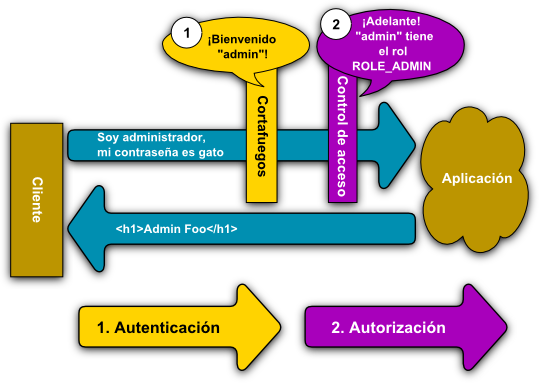
\includegraphics[scale=0.4]{seguridad}
\end{figure}
\begin{block}{}
Se hace uso del algoritmo de encriptación md5 + salt.
  \end{block}
}

\subsection*{Pruebas}

\begin{frame}{Tipos de Pruebas}
  \begin{block}{Pruebas en el desarrollo}
 \begin{itemize}
\item Pruebas unitarias.
\item Pruebas de integración.
\end{itemize}
  \end{block}\pause
  \begin{block}{Pruebas finalizado el desarrollo}
 \begin{itemize}
\item Pruebas de sistema.
\begin{itemize}
\item Pruebas funcionales.
\item Pruebas no funcionales.
\end{itemize}
\item Pruebas de aceptación.
\end{itemize}
  \end{block}
\end{frame}

\begin{frame}{Pruebas de sistema}
  \begin{block}{Pruebas funcionales.}
\begin{itemize}
 \item Se probaron todos los escenarios principales y alternativos de los casos de uso.
\end{itemize}
  \end{block}\pause

  \begin{block}{Pruebas no funcionales.}
	\begin{itemize}
\item Portabilidad - Herramienta online BrowseStack.
\item Mantenibilidad - Estructura de directorios Symfony2.
\item Seguridad - Fundación OWASP.
\item Fiabilidad - Plan de pruebas exhaustivo.
\item Rendimiento - Herramienta online GTmetrix y PigDom(Uso de YuiCompressor, CDN, gzip).
\end{itemize}
  \end{block}
\end{frame}

\begin{frame}{Pruebas de sistema - Portabilidad}
  \begin{figure}[]

\includegraphics[scale=0.15]{Chrome}

\includegraphics[scale=0.15]{Safari}

\includegraphics[scale=0.15]{IE}

\includegraphics[scale=0.15]{Firefox}

\includegraphics[scale=0.15]{Opera}
\end{figure}

  \begin{figure}[]
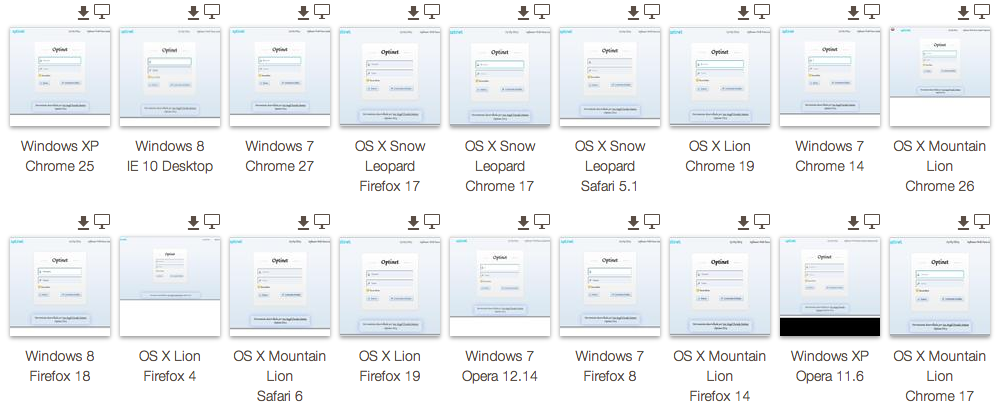
\includegraphics[scale=0.3]{browserstack}
\end{figure}

\end{frame}

\begin{frame}{Pruebas de sistema - Rendimiento}
\begin{itemize}
\item GTmetrix:
  \begin{figure}[]
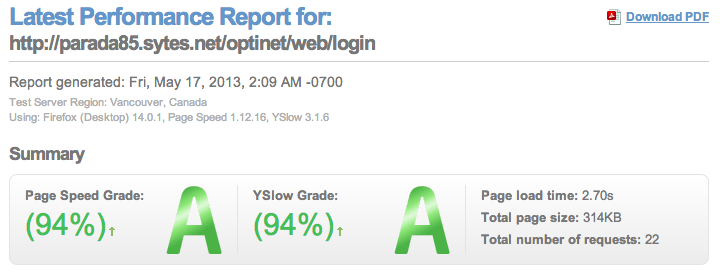
\includegraphics[scale=0.3]{ren}
\end{figure}

\item PigDom
  \begin{figure}[]
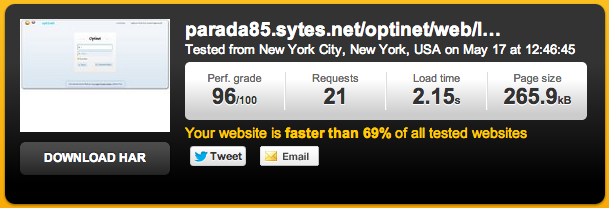
\includegraphics[scale=0.3]{renotro}
\end{figure}
\end{itemize}
\end{frame}

\begin{frame}{Pruebas de aceptación}
Se realizaron diferenciando dos tipos de personas:

\begin{columns}[c]
\column{0.7 \textwidth}
\begin{itemize}
\item Personas con nivel altos de conocimientos informáticos.\\
Compañeros de la universidad con acceso al código de la aplicación.
\begin{itemize}
\item Fallos: Detectaron algunos fallos de seguridad.
\end{itemize}
\item Personas con nivel bajos de conocimientos informáticos.\\
Cliente final y amigos que no dominan la informática.
\begin{itemize}
\item Fallos: Detectaron problemas en usabilidad y diseño.
\end{itemize}
\end{itemize}
\column{0.3 \textwidth}
  \begin{figure}[]

\includegraphics[scale=0.2]{pruebas}
\end{figure}
\end{columns}
\end{frame}


\section{Conclusiones}
\frame{\frametitle{Conclusiones}\tableofcontents[currentsection]}
\subsection*{Objetivos}
\frame{\frametitle{Objetivos}
\begin{block}{Objetivos cumplidos}
\begin{itemize}
\item Se ha construido una aplicación web para gestionar un centro óptico.\checkmark \pause
\item La aplicación gestiona correctamente los productos, proveedores, ventas...\checkmark \pause
\item La aplicación genera informes.\checkmark \pause
\item La aplicación tiene control de las acciones que hacen los usuarios.\checkmark \pause
\item La aplicación es multi-idioma y multi-plataforma.\checkmark \pause
\item La aplicación es segura, fiable y tiene un rendimiento adecuado.\checkmark \pause
\item Plena satisfacción del cliente.\checkmark
\end{itemize}
\end{block}
}

\subsection*{Lecciones aprendidas}
\frame{\frametitle{Lecciones aprendidas}
\begin{block}{Lecciones aprendidas}
\begin{itemize}
\item Lenguajes de programación: HTML, CSS, JavaScript, PHP.
\item Utilización de un framework PHP: Symfony2.
\item Utilización de un framework Javascript: Jquery.
\end{itemize}
\end{block}
}

\section{Posibles mejoras}
\frame{\frametitle{Posibles mejoras}
\begin{block}{Posibles mejoras}
\begin{itemize}
\item Registro de citas por internet.
\item Realización de una aplicación móvil.
\end{itemize}
\end{block}
}

%\section{Bibliografía}
%\frame{\frametitle{Bibliografía}\tableofcontents[currentsection]}
%\frame{\frametitle{Bibliografía}

%\begin{thebibliography}{10}
%\beamertemplatebookbibitems

%\bibitem{11}IBM. \emph{Business Process Execution Language for Web Services 1.1}. 2003.
%\bibitem{20}IBM-OASIS. \emph{Web Services Business Process Execution Language Version 2.0. OASIS Standard}. abril 2007.
%\bibitem{bibliografia1}....
%\end{thebibliography} 
%}


\appendix
\frame
{
  \begin{center}
Gracias por su atención\bigskip 

  \end{center}
}
\end{document}
